\documentclass[tikz,border=4pt]{standalone}
\usepackage{amsmath}
\begin{document}
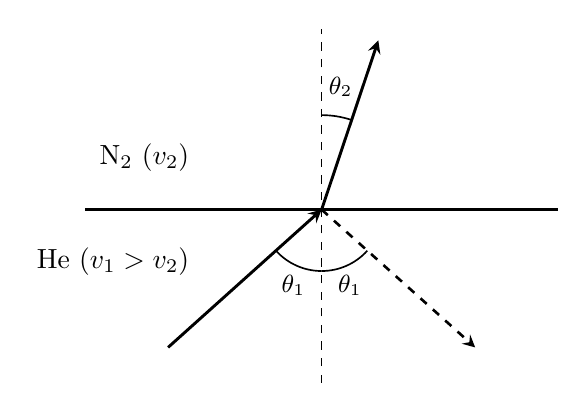
\begin{tikzpicture}[>=stealth, thick, scale=1.0]
  % Membrane along y = 0 and normal along x = 0
  \draw[line width=1.1pt] (-3.0, 0) -- (3.0, 0);
  \draw[dashed, line width=0.6pt] (0, -2.2) -- (0, 2.3);

  % Region labels
  \node[above left] at (-1.55, 0.35) {$\mathrm{N}_2\ (v_2)$};
  \node[below left] at (-1.55, -0.35) {$\mathrm{He}\ (v_1 > v_2)$};

  % Incident ray from bottom-left at theta_1 = 48 deg from normal
  \draw[->, line width=1.05pt] (-1.95, -1.75) -- (0, 0);
  % Reflected ray to bottom-right at theta_1 = 48 deg
  \draw[->, line width=0.95pt, dashed] (0, 0) -- (1.95, -1.75);
  % Refracted ray into N2: theta_2 ~ 18.5 deg (clearly smaller than theta_1 = 48 deg)
  \draw[->, line width=1.05pt] (0, 0) -- (0.72, 2.15);

  % Angle arcs
  % theta_1 incident (between -y axis and incident ray)
  \draw[line width=0.6pt] (0, -0.78) arc (270:222:0.78);
  \node[font=\small] at (-0.36, -0.96) {$\theta_1$};
  % theta_1 reflected (between -y axis and reflected ray)
  \draw[line width=0.6pt] (0, -0.78) arc (270:318:0.78);
  \node[font=\small] at (0.36, -0.96) {$\theta_1$};
  % theta_2 refracted (between +y axis and refracted ray)
  \draw[line width=0.6pt] (0, 1.20) arc (90:71.5:1.20);
  \node[font=\small] at (0.24, 1.56) {$\theta_2$};
\end{tikzpicture}
\end{document}
